%%%%%%%%%%%%%%%%%%%%%%%%%%%%%%%%%%%%%%%%%%%%%%%%%%%%%%%%%%
%   Autoren des Abschnitts:
%   Jakob Kautz
%   Olivier Stenzel
%%%%%%%%%%%%%%%%%%%%%%%%%%%%%%%%%%%%%%%%%%%%%%%%%%%%%%%%%%

% !TEX root =  master.tex
\chapter{Umsetzung - Hardware} \label{umsetzungHW}
\chapterauthor{Jakob Kautz, Olivier Stenzel}

% - Probleme, Schwierigkeiten, Änderungen während der Umsetzung

Nachdem die Planungsphase abgeschlossen war, mussten die Überlegungen umgesetzt werden.
Im Rahmen dieser Arbeit wurde ein Prototyp gebaut, mit dem Ziel möglichst viele der 88 Tasten anzuspielen.
Aufgrund der begrenzten Zeit umfasst der in dieser Arbeit beschriebene Prototyp nur 8 spielbare Tasten,
wäre allerdings ohne weitere Überlegungen auf alle restlichen erweiterbar.
Zusätzlich wurde die Elektronik mit weiteren 32 LEDs so erweitert, sodass das Anspielen von 40 Tasten simulieren kann.


\section{Materialien}
\chapterauthor{Jakob Kautz}
\subsection{Liste der Bauteile}
\begin{table}[htbp]
    \centering
    \begin{tabular}{|m{3.8cm}|m{1.7cm}|m{8cm}|}
        \hline
        \textbf{Bauteil} &  \textbf{Anzahl} & \textbf{Begründung}  \\
        \hline
        Hubmagnete & 88 & jede Taste braucht einen Hubmagneten um angespielt zu werden (Für den Prototypen werden nur 8 verwendet) \\
        \hline
        Stromversorgung & 1 & Externe Stromversorgung für die Aktuatoren, da diese mehr als die 5V Vcc des Arduinos brauchen \\
        \hline
        Arduino & 1 & Kommunikation \\
        \hline
        Breadboard & 10 & Erweiterung der Ausgänge \\
        \hline
        Schaltplatine & 5 & Elektronik für die Aktuatoren\\
        \hline
        Schieberegister & 11 & Weitergabe Signal\\
        \hline
        Kabel (10cm) & 352stck (bzw. $9\cdot40$ in Packs) & Verbindungen in der Schaltung mit Schätzung 4 Kabel pro Hubmagnet\\
        \hline
        Kabel (20cm) & 176stck (bzw.$5\cdot40$ in Packs) & Verbindungen zu den Hubmagneten \\
        \hline
        LEDs & 88 & Tests \\
        \hline
        1kOhm Widerstände & 88 & Sicherheit \\
        \hline
        MOSFET & 88 & Steuerung Strom \\
        \hline
        Feste Anschlussblöcke & 88 & Anschluss von Schaltplatine zu Hubmagnet\\
        \hline
        Angelschnur (1m) & 88 & Verbindung Hubmagnet und Taste \\
        \hline
    \end{tabular}
    \caption{Bauteile Übersicht}
    \label{table:Bauteile}
\end{table}

\subsection{Kostenübernahme}
Die vorher spezifizierte Hardware für den Schaltplan musste für die Erstellung des Prototypen offensichtlich besorgt werden.
Aufgrund der relativ hohen Kosten für eine Studienarbeit, wurde bei einer der betreuenden Firmen angefragt, ob diese die Kosten für das Projekt übernehmen würde.
Damit dies möglich war, wurde ein Kostenvoranschlag gestellt, in welchem die benötigten Materialien mit den geschätzten Kosten aufgeführt wurden.

\begin{table}[htbp]
    \centering
    \begin{tabular}{|m{3.8cm}|m{5cm}|m{5cm}|}
        \hline
        \textbf{Komponente} &  \textbf{Angesetzte Kosten in \euro{}} & \textbf{Tatsächliche Kosten in \euro{}}  \\
        \hline
        Klavier & 200\euro{} & 180\euro{} \\
        \hline
        Arduino & 30\euro{} & 24\euro{} \\
        \hline
        Hubmagnete & 5\euro{} -> 440\euro{} & 13,91\euro{} ->1224.08\euro{} \\
        \hline
        Stromversorgung & 50\euro{} & kostenlos von der Uni bereitgestellt \\
        \hline
        Breadboard & 3\euro{} -> 30\euro{} & 3.43\euro{} -> 34.3\euro{} \\
        \hline
        Schaltplatine & 2\euro{} -> 10\euro{} & 2\euro{} -> 10\euro{}\\
        \hline
        Schieberegister & 0.3\euro{} 3.3\euro{}->  & 8\euro{},da nur in Paket erhältlich\\
        \hline
        Kabel insgesamt & 0.12\euro{}  -> 67\euro{} & 0.12\euro{}  -> 67\euro{}\\
        \hline
        LEDs & Bei der Kostenschätzung nicht mit aufgenommen & 0.10\euro{} -> 8.8\euro{} \\
        \hline
        1kOhm Widerstände & 0.10\euro{} -> 8.8\euro{} & 0.10\euro{} -> 8.8\euro{} \\
        \hline
        MOSFET & 0.9\euro{} -> 79.2\euro{} & 0.66\euro{} -> 58,08\euro{} \\
        \hline
        Feste Anschlussblöcke & Bei der Kostenschätzung nicht mit aufgenommen  & 10\euro{}\\
        \hline
        Verbindung gesamt & 100\euro{} & 120\euro{} \\
        \hline
    \end{tabular}
    \caption{Übersicht der Kosten}
    \label{table:kosten}
\end{table}

Der Kostenanschlag erwies sich im Laufe des Projektes als (teils) unrealistisch. Dies lag insbesondere an der Anforderung
der Firma. Die Schätzung der Kosten basierte auf Anbietern, bei welchen die Materialien möglichst günstig zu kaufen sind.
Durch Firmenreglungen mussten diese allerdings alle bei Conrad oder Reichelt
gekauft werden. Diese Anbieter verkaufen die Materialien für sehr viel mehr Geld.
Hierbei ist allerdings zu erwähnen, dass die Kostenschätzung passend gewesen wäre, wenn die Anbieter frei wählbar wären.

\section{Prototypenbau} \label{Prototyp}
\chapterauthor{Olivier Stenzel}
Ursprünglich sollte der Aufbau des in Kapitel \ref{subsec:schaltplan} spezifizierten Schaltplans via Steckbrettern und
Jumperkabeln umgesetzt werden.
Zu Beginn wurde dies auch so umgesetzt. Das Problem welches dadurch entstand, war, dass die gewählten Platinen den
benötigten Stromfluss nicht aushalten.\newline
Jeder Aktuator - also jede gedrückte Taste - zieht einen Strom von 0.7A. Um das Projekt möglichst sinnvoll umzusetzen,
sollte der Aufbau mindestens 10 Tasten gleichzeitig drücken können, was bedeutet, dass der Aufbau mindestens 7.0A
Stromfluss problemlos ausstehen muss.

Aus diesem Grund wurde die gesamte Schaltung, die nach dem Schieberegister kommt, auf einer Lochrasterplatine fest gelötet.
Hierfür wurde ein 3mm starker Draht für die Stromversorgung verwendet. \newline
Es wurde bei den Kabeln und Steckplatinen damit gerechnet, dass maximal 20 Aktuatoren Gleichzeitig gespielt werden.
Da ein Großteil der Stücke für eine:n einzelne:n Pianist:in geschrieben wurde, kann davon ausgegangen werden, dass
generell nicht mehr als 10 Tasten Gleichzeitog gespielt werden müssen - tendenziell weniger. Die restlichen 10
Tastendrücke die dazu gerechnet wurden, sind lediglich eine Versicherung.

\subsection{Verbindung Tasten und Aktuatoren} \label{subsec:VerbindungTastenAktuatoren}
\chapterauthor{Olivier Stenzel}

Wie in Kapitel \ref{subsec:konzeptionhw-ansteuerungskonzept} beschrieben wurde sich für ein Ziehen der Tasten entschieden.
Dieses Ziehen wird technisch mittels Hubmagneten umgesetzt. \newline

Dieses Kapitel beschreibt wie und wo die Hubmagnete am Klavier und den Tasten befestigt werden.
Zusätzlich wird der Aufbau im Verlauf des Kapitels bezüglich Reibung und Genauigkeit beim Ansteuerns der Tasten weiter verbessert.
\newline

Die Grundidee ist, mittels einer Schnur, oder Ähnlichem die Tasten mit den Hubmagneten zu verbidnen.
Diese sollen dann an der Schnur, und somit an der Taste ziehen, welche wiederrum den Hammer an die Saite schlagen lässt.

Die Schnur wird mittels eines waagerechten Loches in der Taste, an dieser zu befestigen.
Die Position an der Taste kann nicht frei gewählt werden.
Es muss darauf geachtet werden, dass das Loch möglichst am Ende der Taste angebracht wird, um einen größeren Hebeleffekt zu erzeugen.
Zusätzlich ist es wichtig, dass das Tastenbrett unter der Taste an der Position gut durchzubohren ist.
Eine optische nicht notwendige Eigenschaft wäre, dass das Seil beim spielen nicht von oben gesehen wird.
In Abbildung \ref{img:Tastenbohrung} sieht man, wie die Montage umgesetzt wurde.
Mit rot ist das gebohrte Loch gekennzeichnet, durch das ein Seil (in grün dargestellt) geführt wird.

\begin{figure}[htbp]
    \centering
    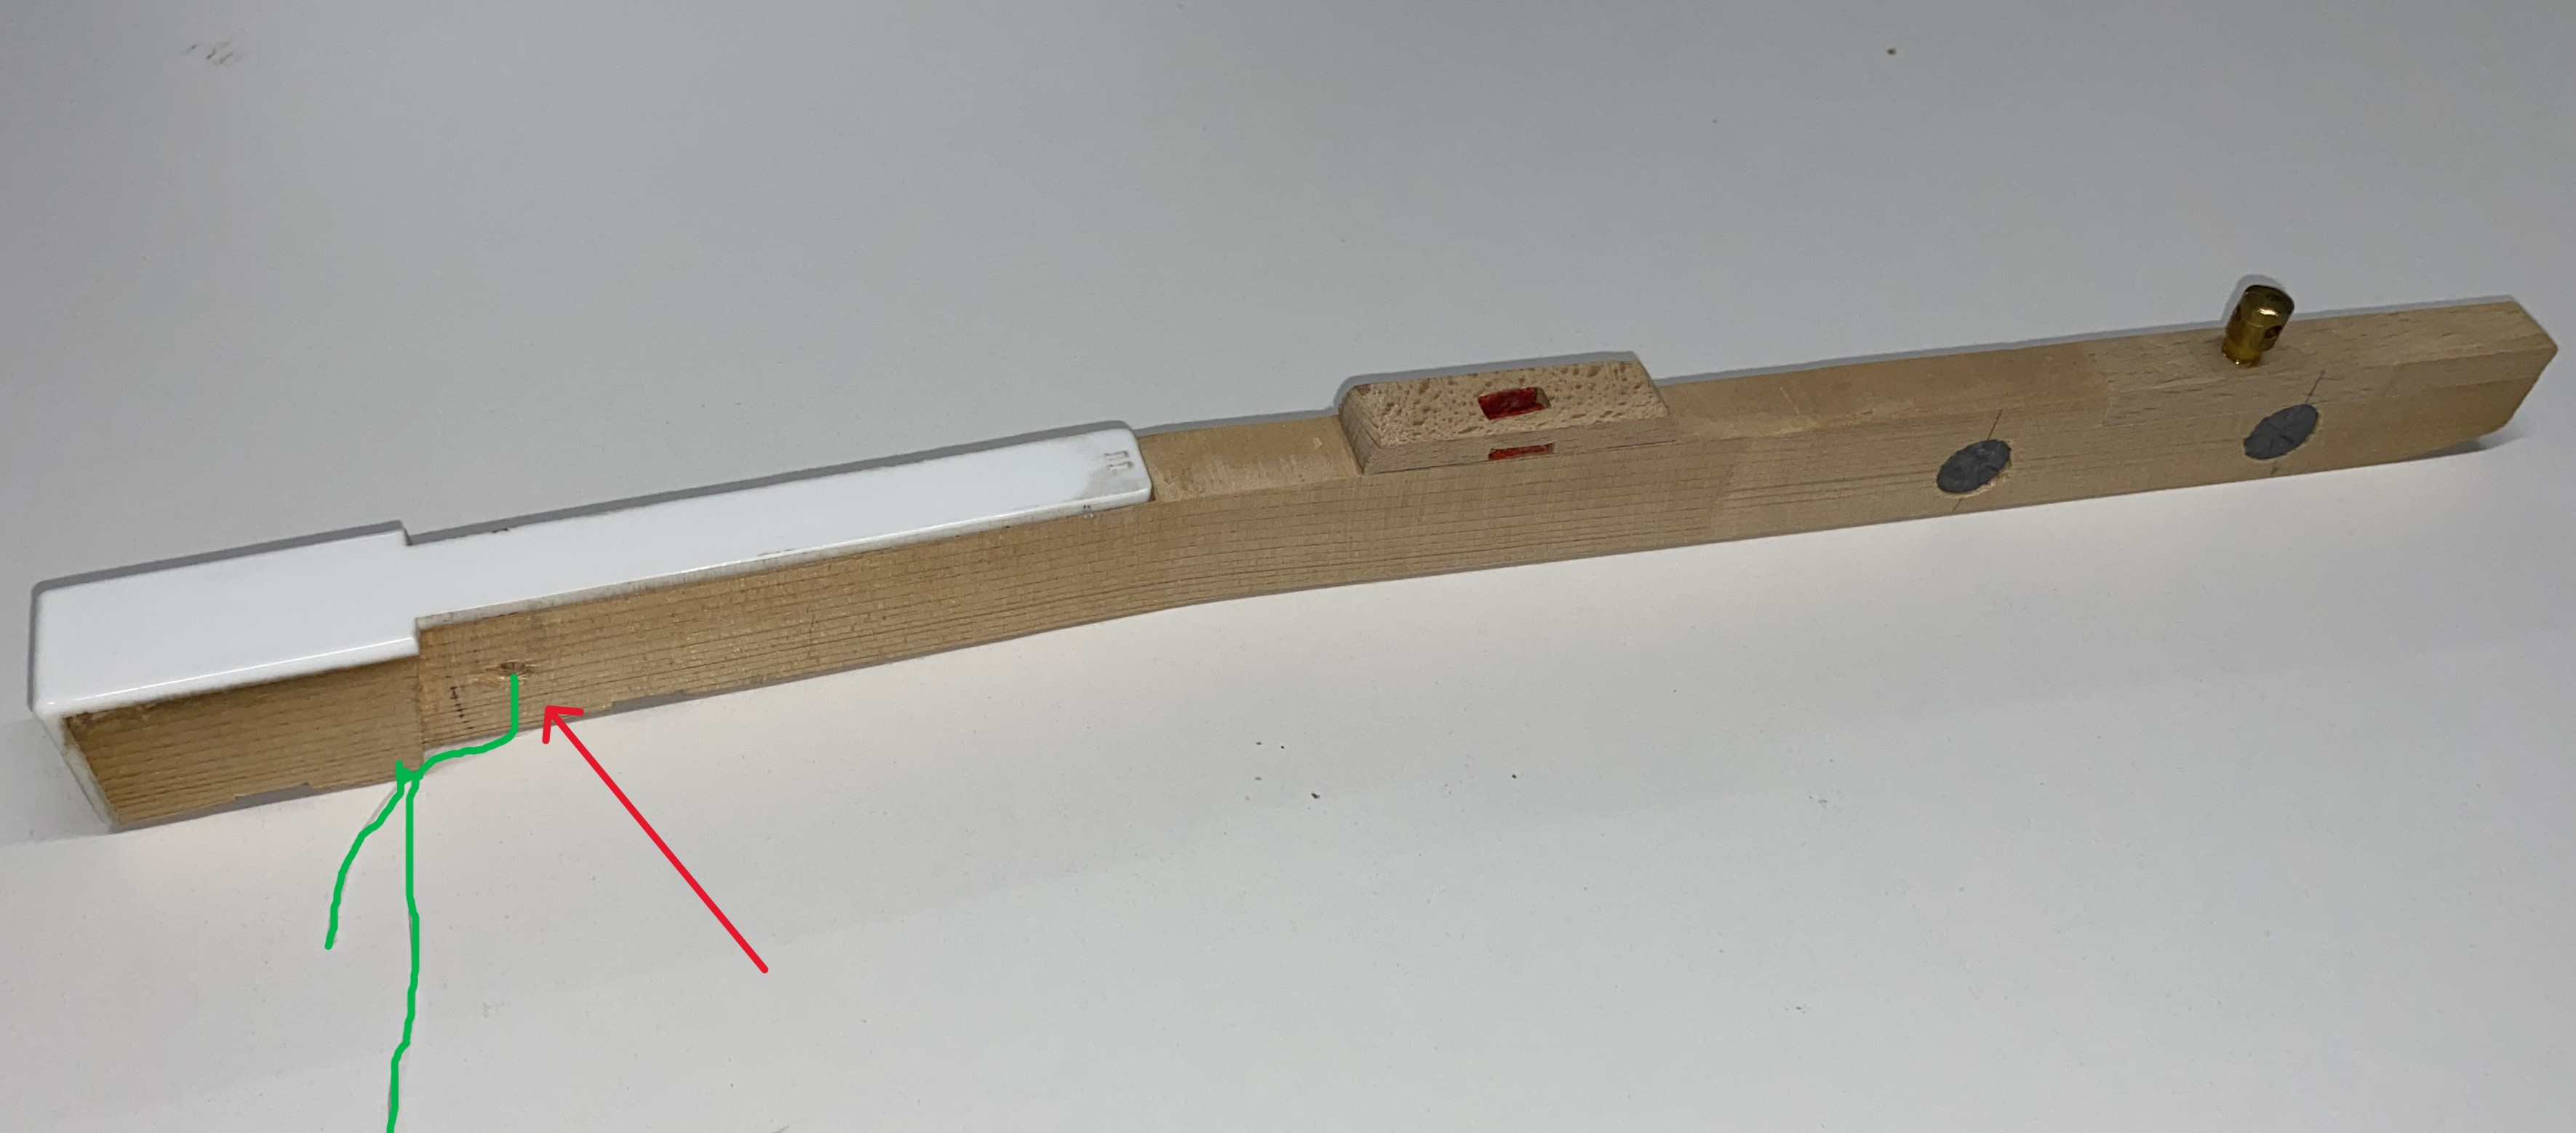
\includegraphics[width=8cm]{img/Taste_schraeg.jpg}
    \caption{Tastenbohrung}
    \label{img:Tastenbohrung}
\end{figure}


Anschließend wird jede Schnur einzelnd in den Fußraum geführt.
Dafür werden senkrechte Löcher (rot in Abbildung \ref{fig:klaviatur}) in den Klaviaturbalken (bzw. Tastenbrett),
worauf die Tasten liegen, gebohrt.

\begin{figure}[htbp]
    \centering
    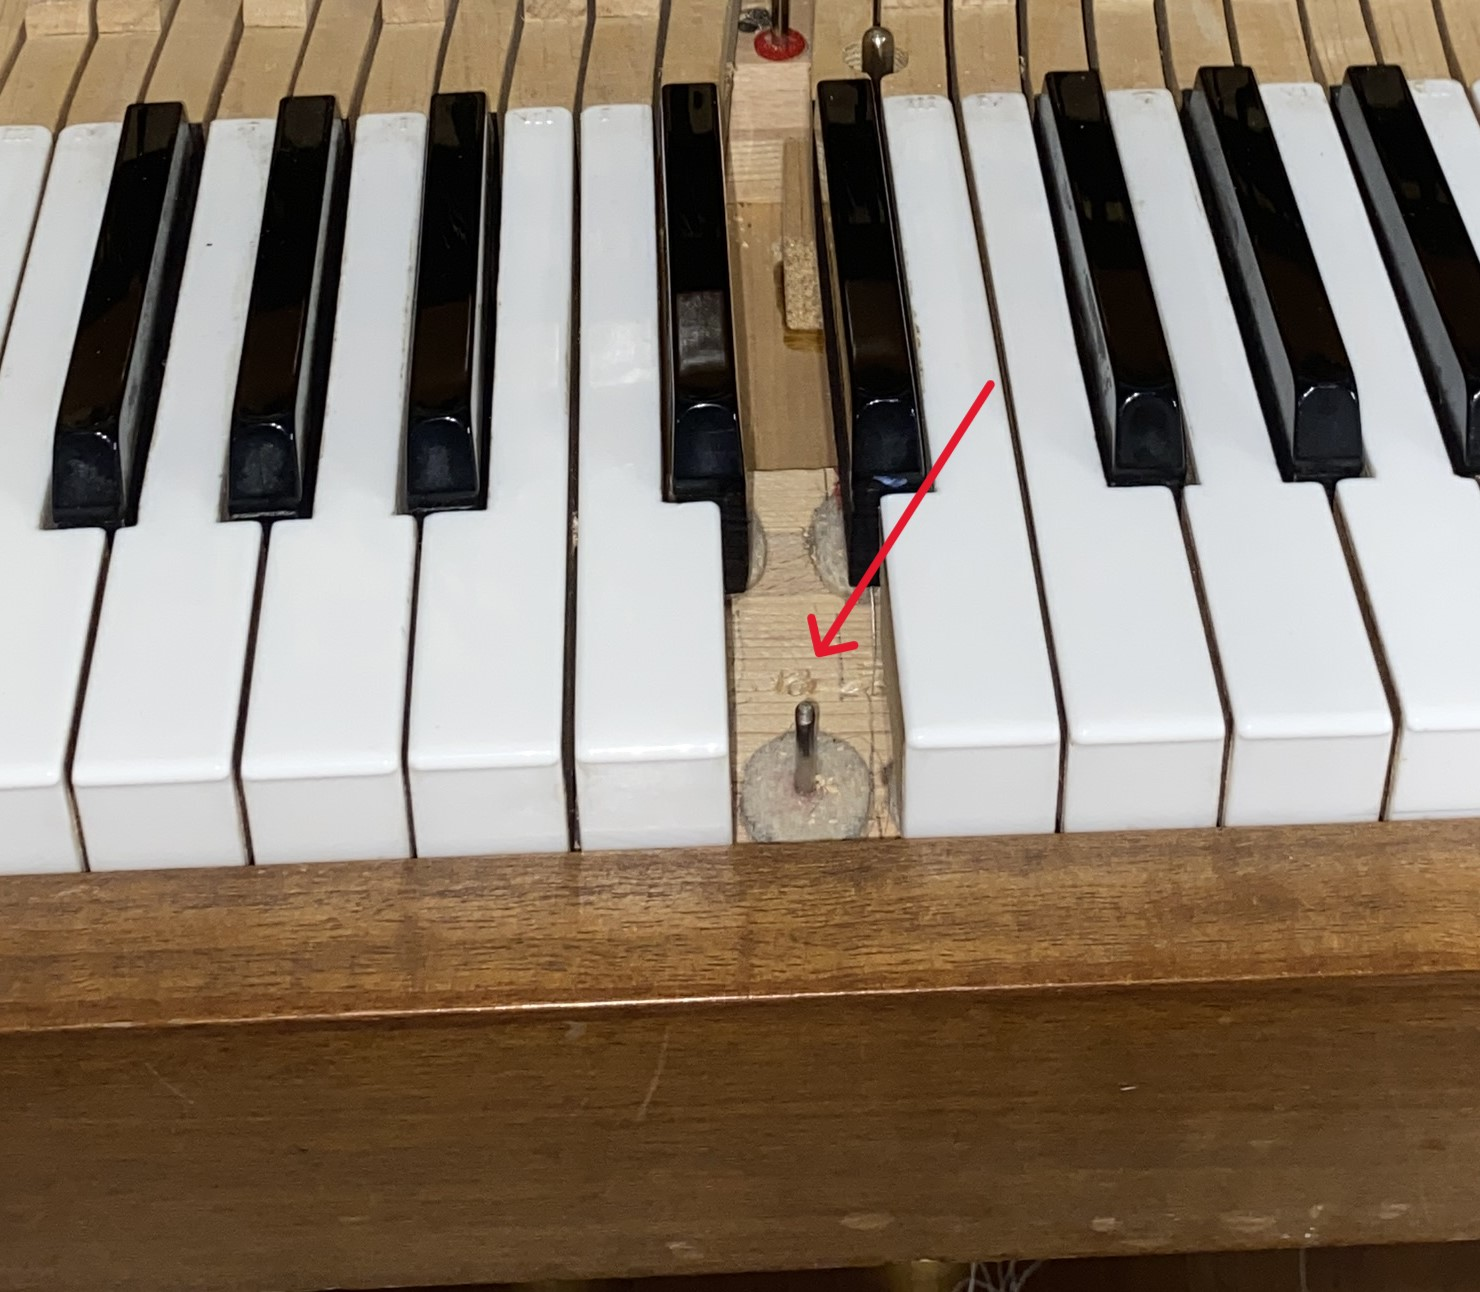
\includegraphics[width=5cm]{img/Klaviatur.jpg}
    \caption{Bohrung durch das Tastenbrett}
    \label{fig:klaviatur}
\end{figure}

\subsubsection{Anordnung der Aktuatoren}

Die Idee ist, die Hubmagnete parallel zur Klaviatur zu befestigen, um die Tasten möglichst senkrecht nach unten ziehen zu können.
Hierfür müssen folgende Aspekte berücksichtigt werden:

\begin{enumerate}
    \item Breite der Hubmagnete
    \item Hitzeentwicklung
    \item Seilführung
    \item Stabilität
    \item Modularität
\end{enumerate}

Ein Hubmagnet hat die Maße 2,5 cm x 6 cm.
Das Tastenbrett für 88 Tasten ist allerdings nur 140 cm breit, wodurch pro Tastenansteuerung nur ca. 1,6 cm zur Verfügung stehen.
Bildet man zwei Hubmagnetreihen übereinander, hat jede Tastenansteuerung 3,20 cm Platz.

Durch die 7mm Abstand ist eine Wärmeabfuhr über die Luft in geringem Ausmaß möglich.
Alle Seile werden pro Hubmagnetreihe, parallel zwischen Tasten und Hubmagneten verbunden.

Die Hubmagnete direkt unter dem Tastenbrett zu befestigen wäre eine triviale Lösung, würde allerdings auf Kosten der Spielbarkeit (siehe Anforderung 1 in Kapitel \ref{Zielstellung}) gehen.
Um also die Beinfreiheit der Pianist:in zu gewährleisten
werden die Hubmagnete am Korpus des Klaviers (untere Frontplatte) befestigt.

Um die Austauschbarkeit der Komponenten zu verbessern, werden die Hubmagnete nicht direkt an der unteren Frontplatte,
sondern auf zwei Pressspanplatten (ca. 70 cm x 25 cm) befestigt, welche an vier Punkten mit dem Klavier verschraubt werden können(siehe Abb. \ref{fig:BefestigungHubmagnete}).
In diesem Prototyp wird die Verschraubung an das Klavier nicht genutzt, um an Flexibilität zu gewinnen.

\begin{figure}[htbp]
    \centering
    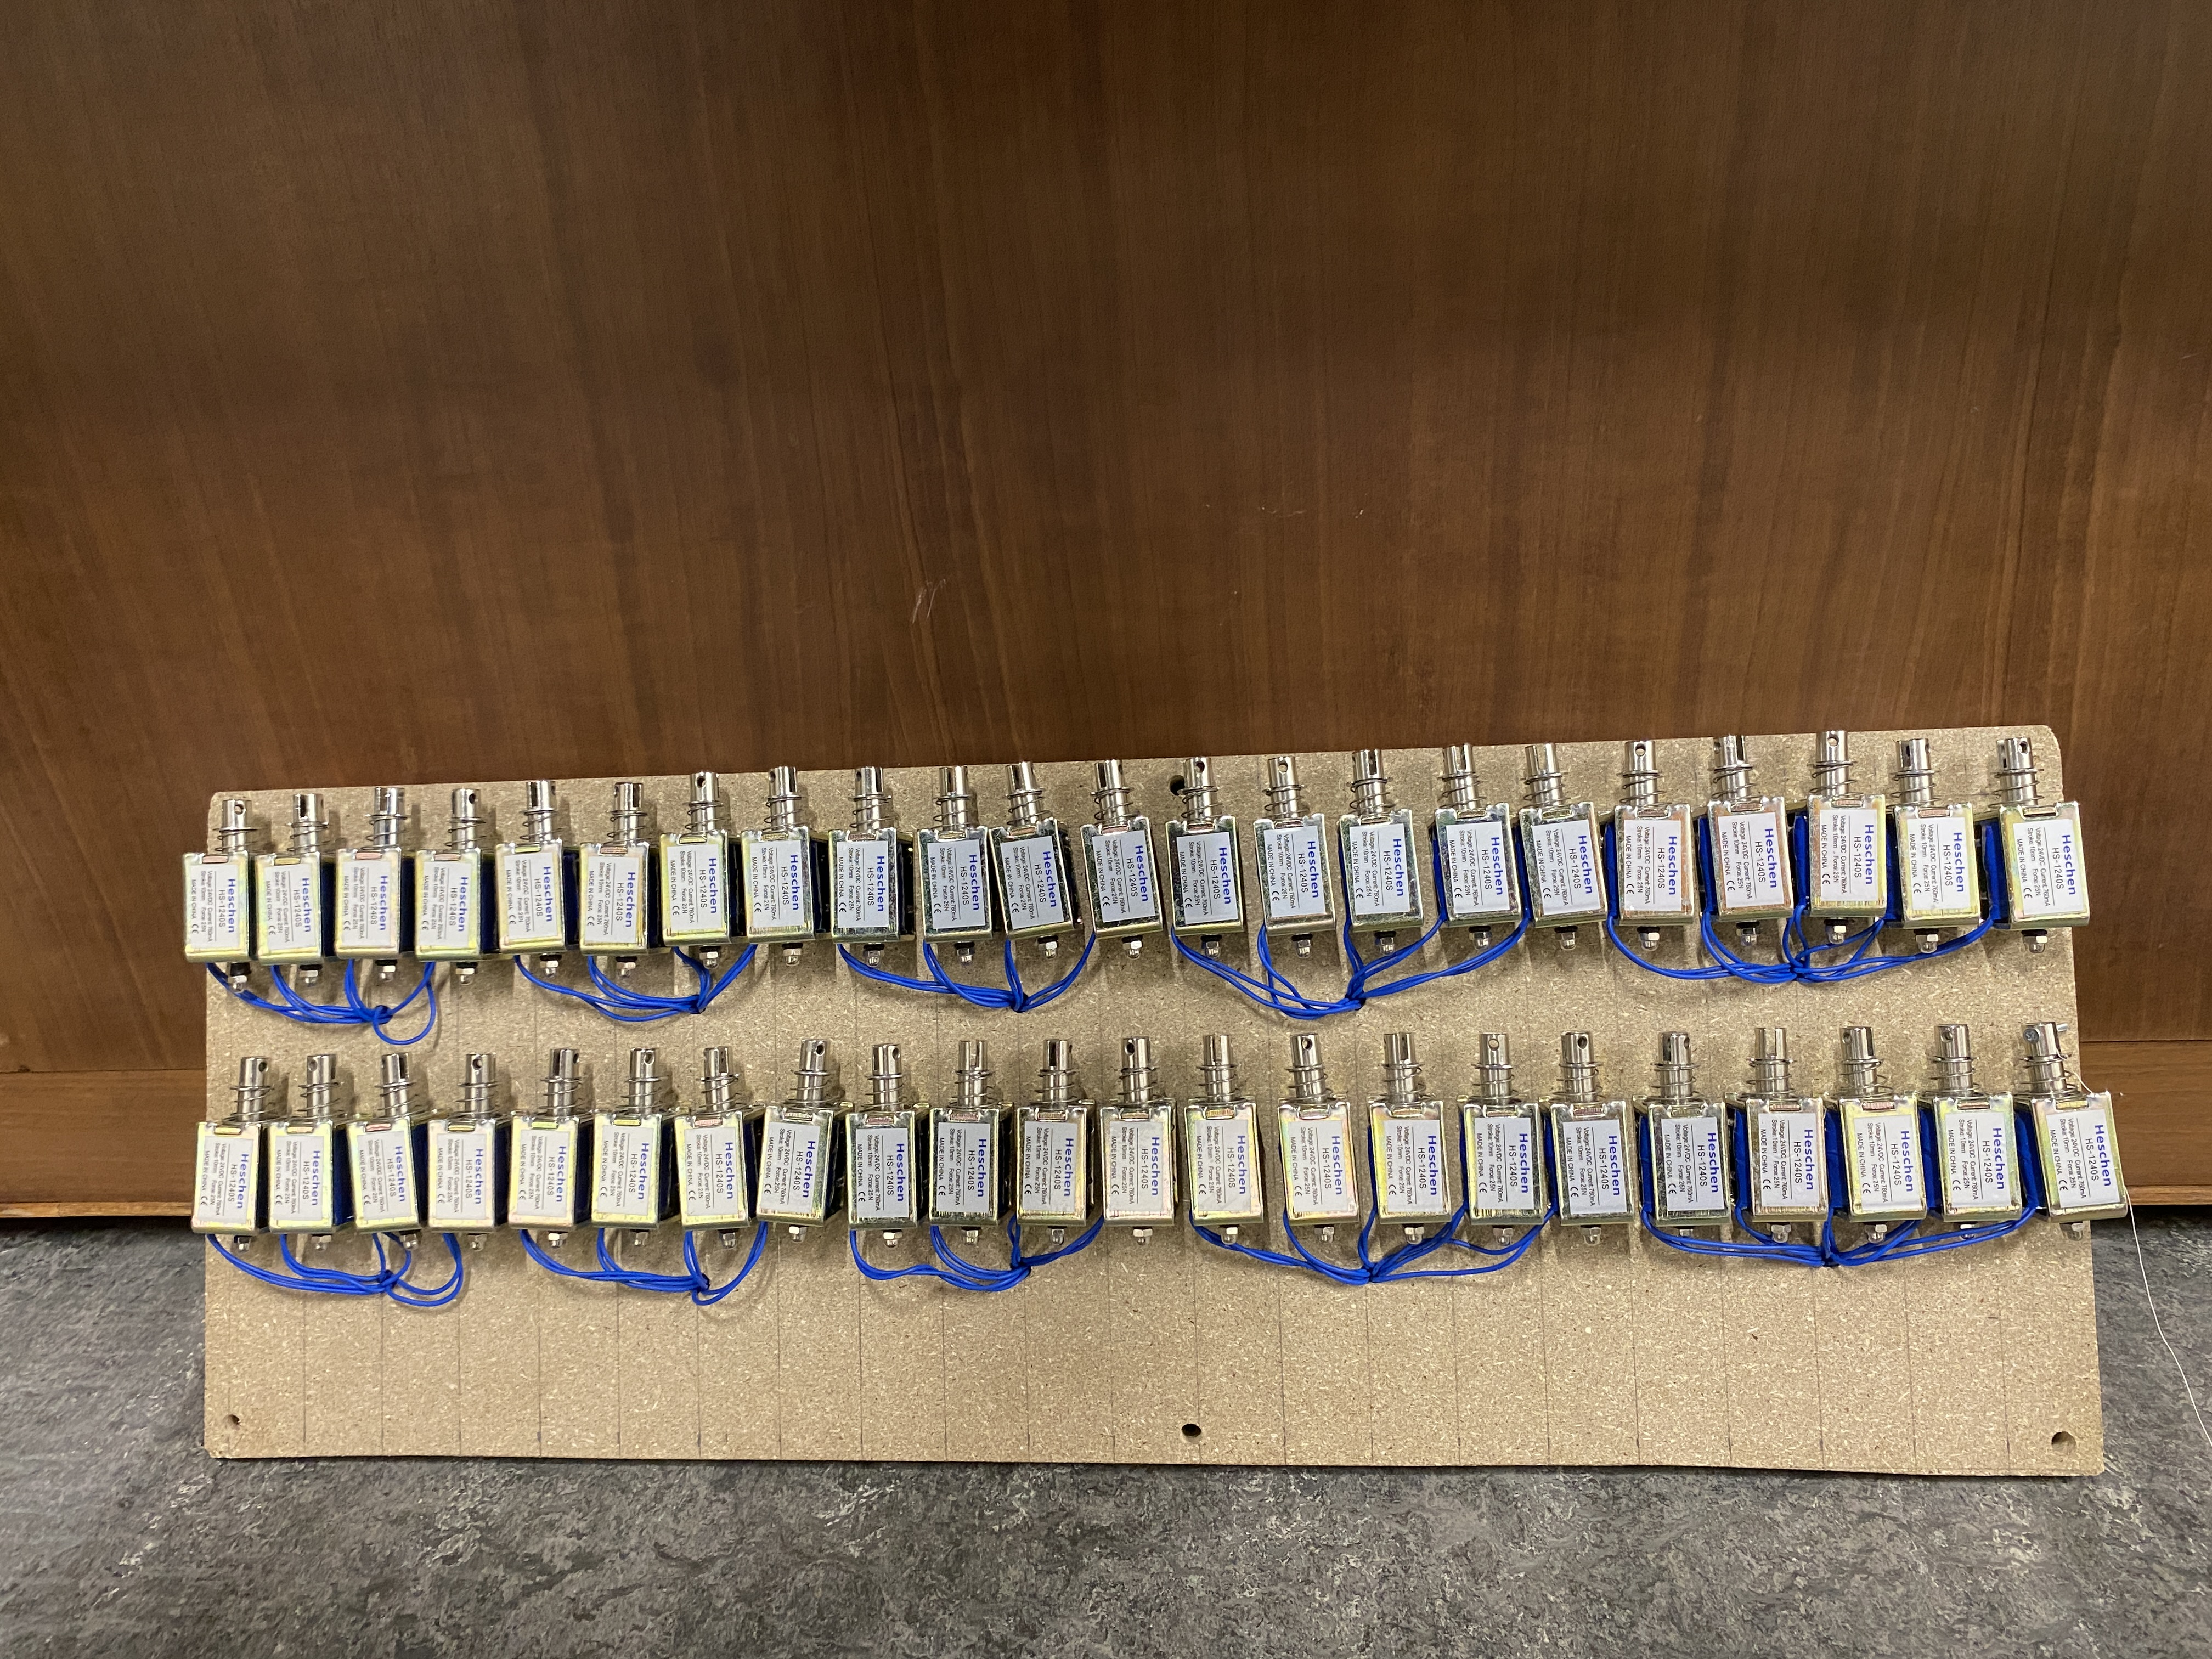
\includegraphics[width=5cm]{img/Magnetbrett.jpg}
    \caption{Befestigung der Hubmagnete}
    \label{fig:BefestigungHubmagnete}
\end{figure}

\subsubsection{Seilführung}

Würde man die Seile von den Tasten direkt zu den Hubmagneten führen,
hätte man deutliche Hub-Verluste und könnte unter Umständen die Tasten nicht mehr ausreichend stark betätigen, um einen Ton zu erzeugen.
\newline
In den folgenden Abbildungen ist die seitliche Ansicht des Klaviers gezeichnet.
Dabei repräsentieren der schwarze bzw. weiße Block jeweils eine schwarze bzw. weiße Taste.
Der grüne und pinke Strich stehen für die Seile, die den Hubmagneten mit dem Loch in der Taste verbinden.
Unten links sind die zwei übereinanderliegenden Solenoid-Reihen abgebildet.
Der schwarze Strich repräsentiert den Stab im Hubmagneten.
\newline
Abbildung \ref{img:kUmlenkung_locker} zeigt den intuitiven Aufbau mit ausgeschaltetem Solenoid und entsprechend entspanntem Seil und.
Abbildung \ref{img:kUmlenkung_gezogen} zeigt den selben Aufbau mit dem Unterschied, dass der Solenoid hier angezogen ist.

\begin{figure}[htbp]
    \centering
    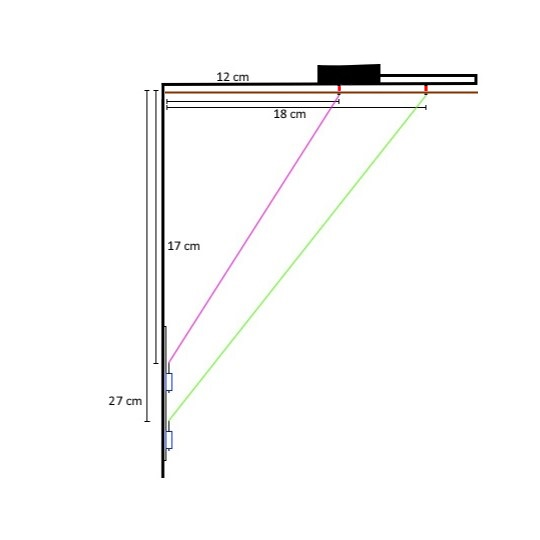
\includegraphics[width=6cm, height=8cm]{img/Umlenkung_locker}
    \caption{Taste locker ohne Umlenkung}
    \label{img:kUmlenkung_locker}
\end{figure}

\begin{figure}[htbp]
    \centering
    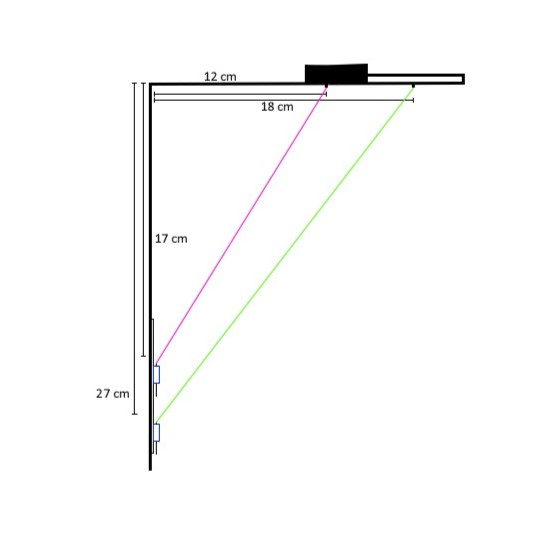
\includegraphics[width=6cm, height=8cm]{img/Umlenkung_gezogen}
    \caption{Taste gezogen ohne Umlenkung}
    \label{img:kUmlenkung_gezogen}
\end{figure}

Mit diesem intuitiven Aufbau funktioniert das Betätigen der Tasten nicht, da diese nicht weit genug heruntergezogen werden.
Um den gesamten Hub des Magneten zu Nutzen und an die Taste weiterzugeben, müssen Umlenkungen eingebaut werden.
Mittels dieser Umlenkung, die mit einem PVC-Rohr umgesetzt werden kann, werden die Seile so geführt, das sie senkrecht auf die Hubmagnete fallen.
Somit wird die Tiefe, mit der die Tasten gedrückt werden, wieder auf annähernd 1 cm erhöht, was dem Hub des Magneten entspricht..

\begin{figure}[htbp]
    \centering
    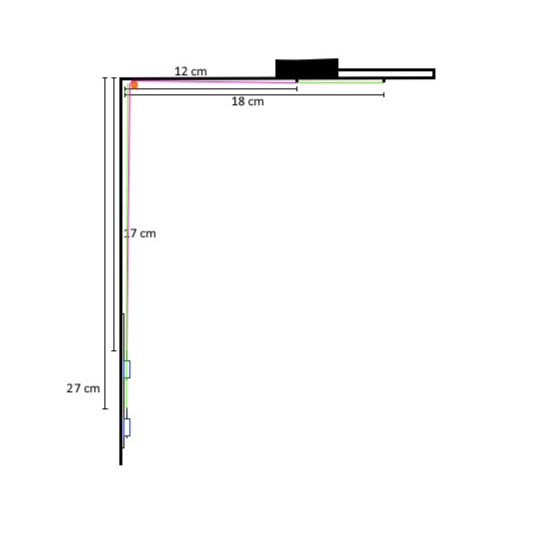
\includegraphics[width=6cm, height=8cm]{img/mitUmlenkung_locker}
    \caption{Taste mit Umlenkung}
    \label{img:mitumlenkung_locker}
\end{figure}


\newpage
Dies kann auch mathematisch bewiesen werden:
\newline geg.:
\newline Distanz zwischen dem Tastenbrett und der unteren Reihe Hubmagnete h = 27 cm
\newline Distanz zwischen der unteren Frontplatte und dem zum Loch im Tastenbrett t = 18 cm

Gesucht ist die Differenz der Längen zwischen dem Tastenbrett und dem Hubmagneten, wenn die Tasten (nicht-)gedrückt sind.
Diese ist in Zeichnung \nameref{img:kUmlenkung_locker} und \nameref{img:kUmlenkung_gezogen} rot gekennzeichnet.
\newline $ht_{entspannt}$ beschreibt die Seillänge zum Tastenbrett im entspannten Zustand
\newline $ht_{entspannt}$ = $\sqrt {h^{2} + t^{2}}$ = 32.45 cm
\newline $ht_{gespannt}$ = $\sqrt {(h + 1)^{2} + t^{2}}$ = 33.29 cm


Die Differenz zwischen $ht1_{gespannt}$ und $ht1_{entspannt}$ (bzw. ht2) beschreibt die Tiefe,
die eine Taste gedrückt werden kann, wenn der Hub des Magnetens 1 cm beträgt.
\newline Diese beträgt also ohne Umlenkung nur 0.84 cm.
Mit der Umlenkung (siehe \nameref{img:mitumlenkung_locker})

Um also die Intensität des Tastendrucks besser steuern zu können und um die Haltbarkeit des Materials zu verlängern,
sollte die Reibung am Seil möglichst gering gehalten werden.
Dazu können mittels Rohren, welche waagerecht unter dem Klaviaturbalken entlang der Löcher montiert werden können (siehe Abbildung \ref{fig:fussraum}), die Seile umgelenkt und
entlang der Verkleidung zur unteren Frontplatte des Klaviers geführt werden.
Das hat den positiven Nebeneffekt, dass die Pianist:innen nicht durch Platzmangel im Beinbereich eingeschränkt sind.


\begin{figure}[htbp]
    \centering
    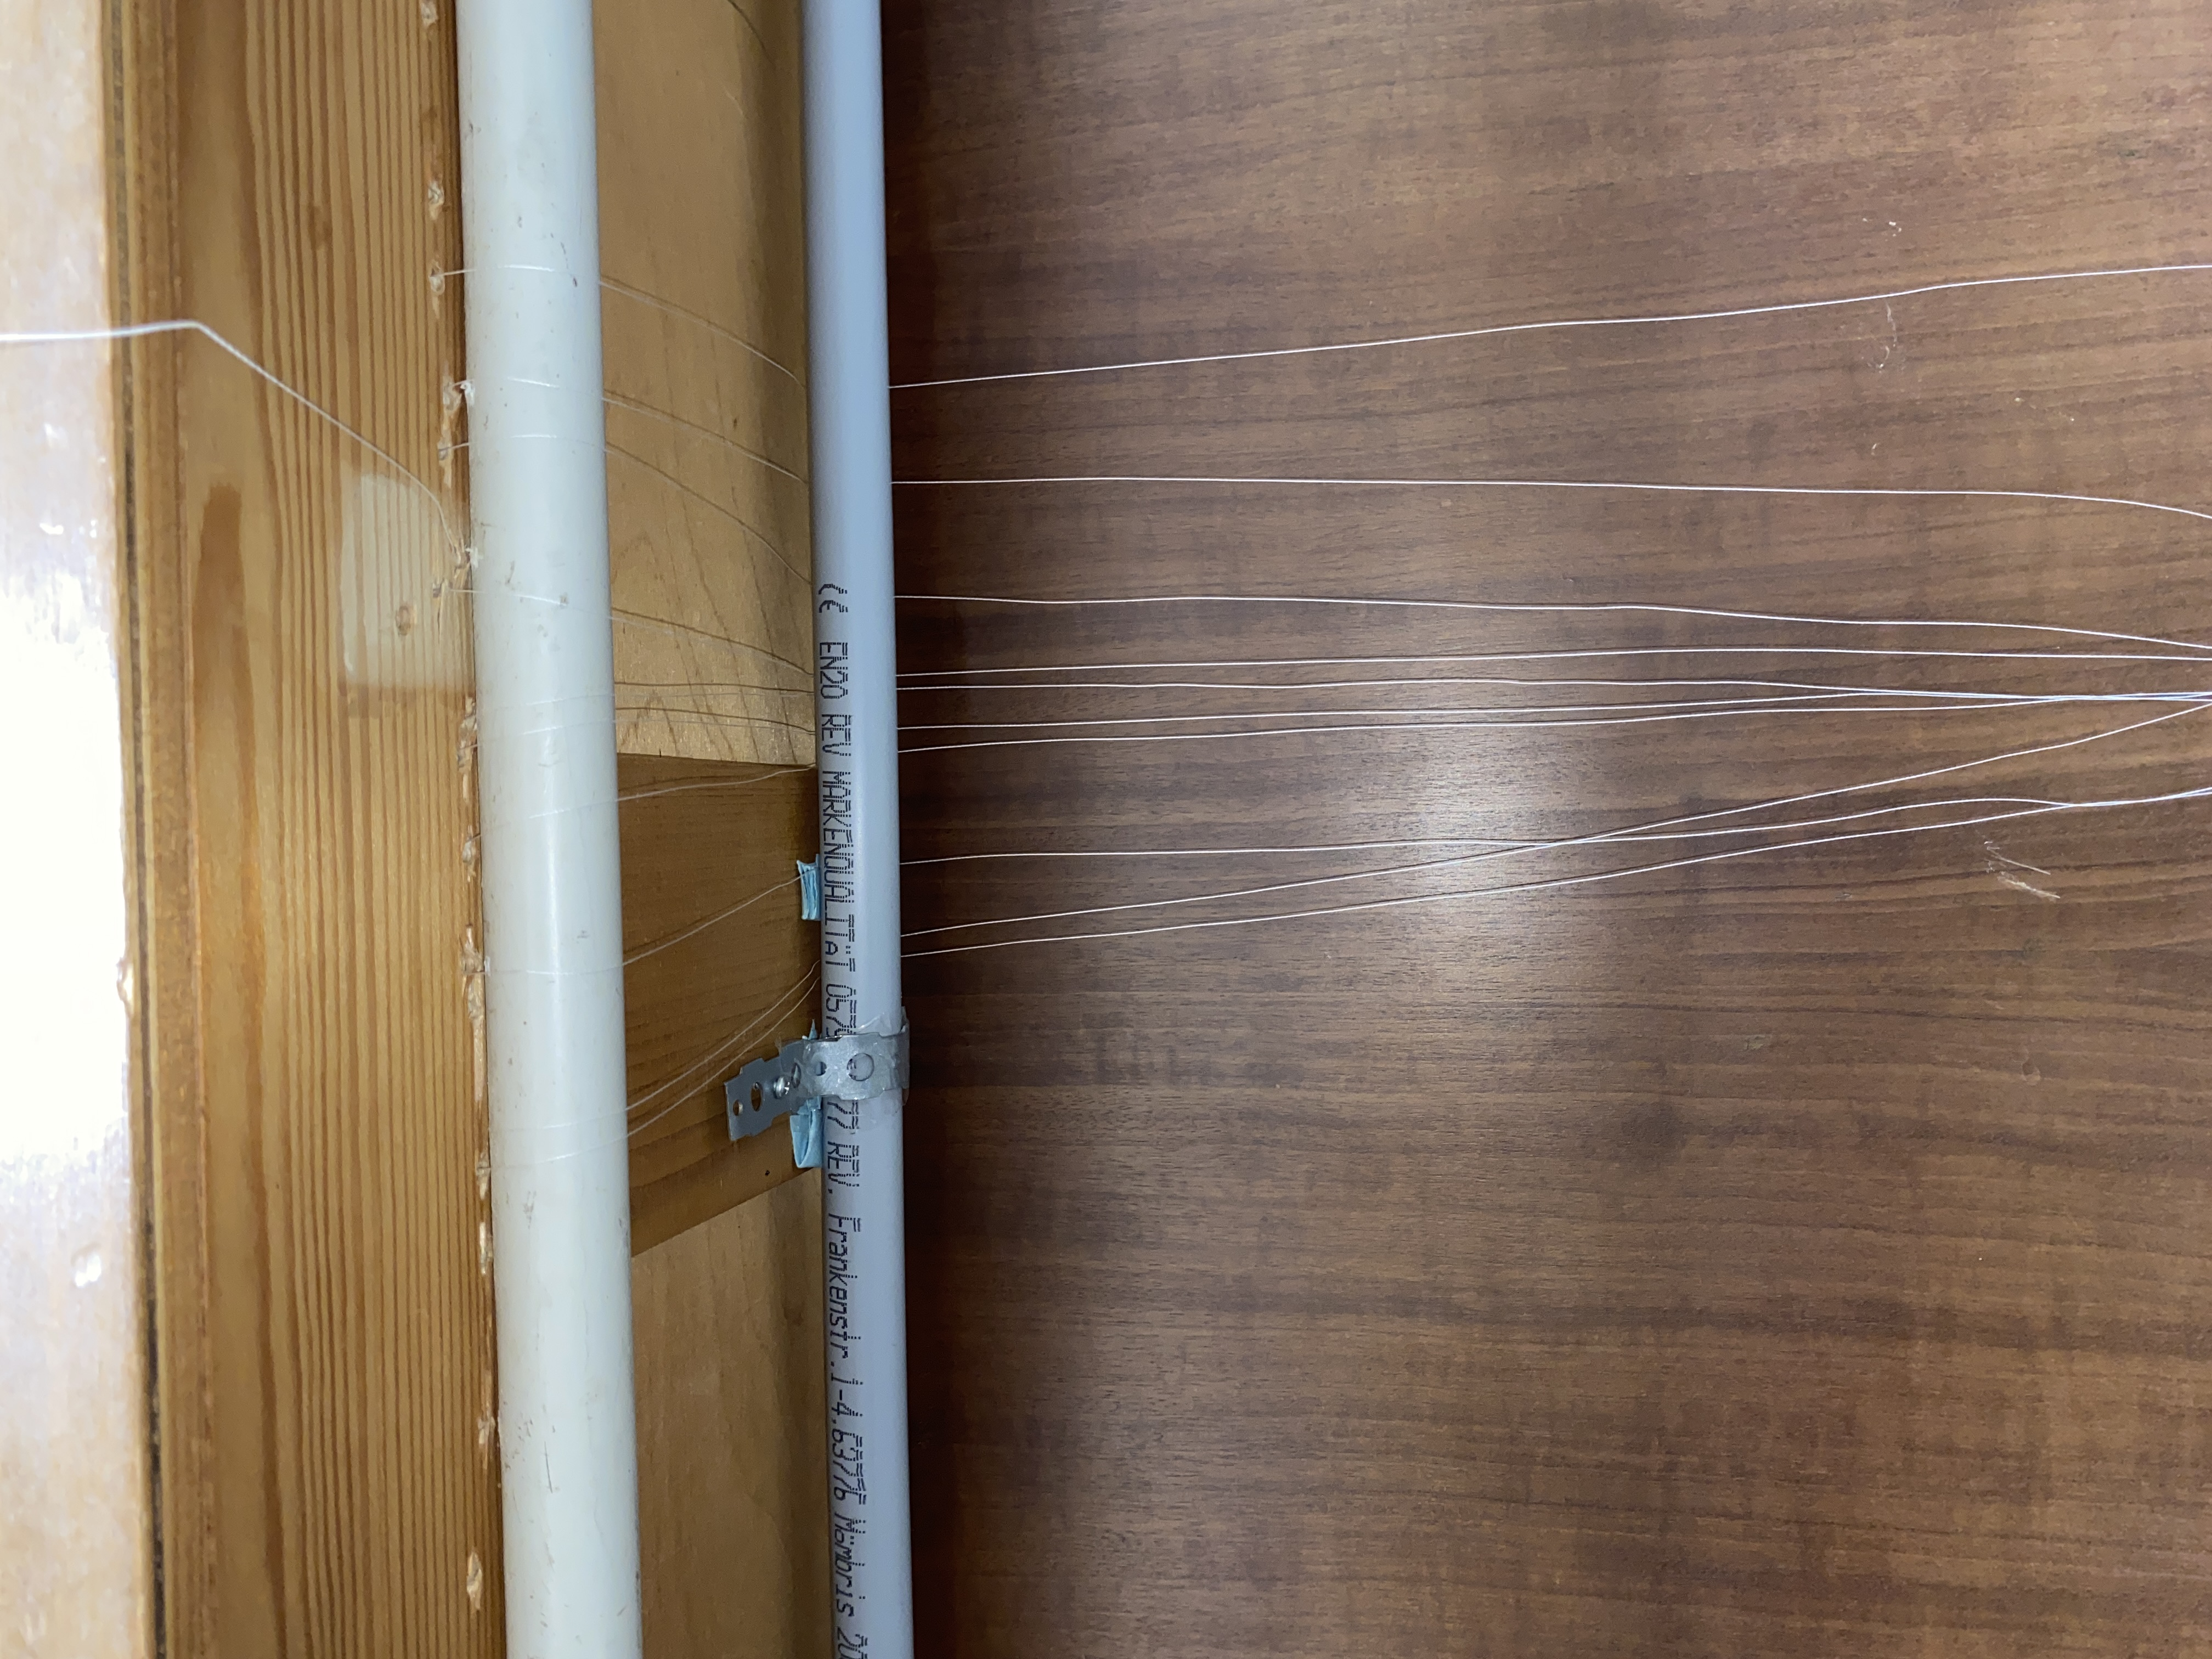
\includegraphics[width=5cm,angle=-90]{img/Fussraum.jpg}
    \caption{Fußraum des Klaviers}
    \label{fig:fussraum}
\end{figure}


\subsubsection{Auswahl des Seils}

Wie eben beschrieben wird das Ziehen durch ein Seil ermöglicht.
Dafür wird ein leichtes, formbares, unelastisches und dehnungsresistentes Material benötigt, welches die Hubmagnete mit den Tasten verbindet.
Je leichter das Material ist, desto weniger geht die Genauigkeit der Kraftübertragung zwischen den Magneten und den Tasten verloren.
Durch die Formbarkeit kann der Knoten sehr eng an der Taste geschnürt werden, wodurch das Ansprechverhalten schneller erfolgen kann.
Da die Anschläge ruckartige Bewegungen sind, ist es wichtig ein unelastisches Seil zu verwenden.
Um häufiges Nachspannen oder Austauschen des Seils entgegenzuwirken, sollte dies so dehnungsresistent wie möglich sein.

\paragraph{Nähgarn}

Als Erstes wurde Nähgarn, welches zur Hand war, getestet.
Auch doppelt verlegt hielt es der ruckartigen Ziehbewegung (mit 25N) des Hubmagnetens nicht stand.
Vier Fäden funktionierten zu Beginn gut, leierten allerdings schnell aus.

\paragraph{Nylonsaiten}

Als Nächstes wurde die g-Saite einer Gitarre verwendet.
Durch den höheren Durchmesser und das stärkere Material riss und leierte die Saite nicht aus.
Da die Saite kaum Flexibilität liefert, war die Befestigung an der Taste jedoch äußerst schwierig.
Beim Ziehen des Magnetens wurde erst die lockere Schlaufe an der Taste gestreckt, wodurch nicht der vollständige Hub des Magnetens auf die Taste übertragen wurde.

\paragraph{Angelschnur}

Mit einer kurzen Auseinandersetzung mit dem Angelzubehör konnte schnell eine geeignetere Schnur gefunden werden.
Genauer handelt es sich um eine geflochtene Schnur aus Polyethylene.
Mit einem Durchmesser von 1.6 mm ist sie nicht nur sehr dünn und flexibel, sondern kann auch bis zu 7 kg standhalten.
Nach ausgiebigem Testen ist eindeutig, dass die Angelschnur die Anforderungen erfüllt.
Damit ist nun auch das Spielen des Forellenquintetts von Schubert ein Leichtes.

\subsection{Klangdämpfung der Aktuatoren}

\chapterauthor{Olivier Stenzel}

Die Hubmagnete machen beim Anschlagen laute \enquote{Klack} Geräusche, welche von der Melodie des Klaviers ablenken.
Genauer handelt es sich um den Metall-Anker, der gegen das Ende des Metall-Gehäuses stößt.
Auch hierfür gab es mehrere Ideen und Tests, um das Geräusch zu dämpfen:

\subsubsection{Isolierfolie}

Die erste Überlegung war die Auskleidung des Innenraums der Hubmagnete mit Isolierfolie.
Diese Idee wurde wieder verworfen, da das Wissen über die Hitzeentwicklung zu diesem Zeitpunkt noch zu gering war, um sicherzustellen, dass die Isolierung dem standhält. % "dem" meint die Hitzeentwicklung? Dann müsste es "ihr" sein.

\subsubsection{Gummi-Stopper}

Die nächste Idee war das Limitieren des Schlags durch Dichtungsringe aus Gummi
zwischen Anker und dem äußeren Gehäuse.
Da für die Befestigung keine zufriedenstellende Lösung gefunden wurde, wurde auch diese Idee verworfen.

\subsubsection{Schaumstoff}

Wie im Abbildung \ref{fig:schaumstoff} zu sehen ist, wurde die \enquote{Gummi-Stopper}-Idee durch den Einsatz von Schaumstoff leicht modifiziert. \newline
+ Klopfgeräusch wird vollständig verhindert \newline
- Durch den Schaumstoff wird 1mm des Hubs nicht verwendet, weshalb nur noch 9mm übrig bleiben \newline
- Der Aufbau ist optisch nicht besonders ansprechend

\begin{figure}[htbp]
    \centering
    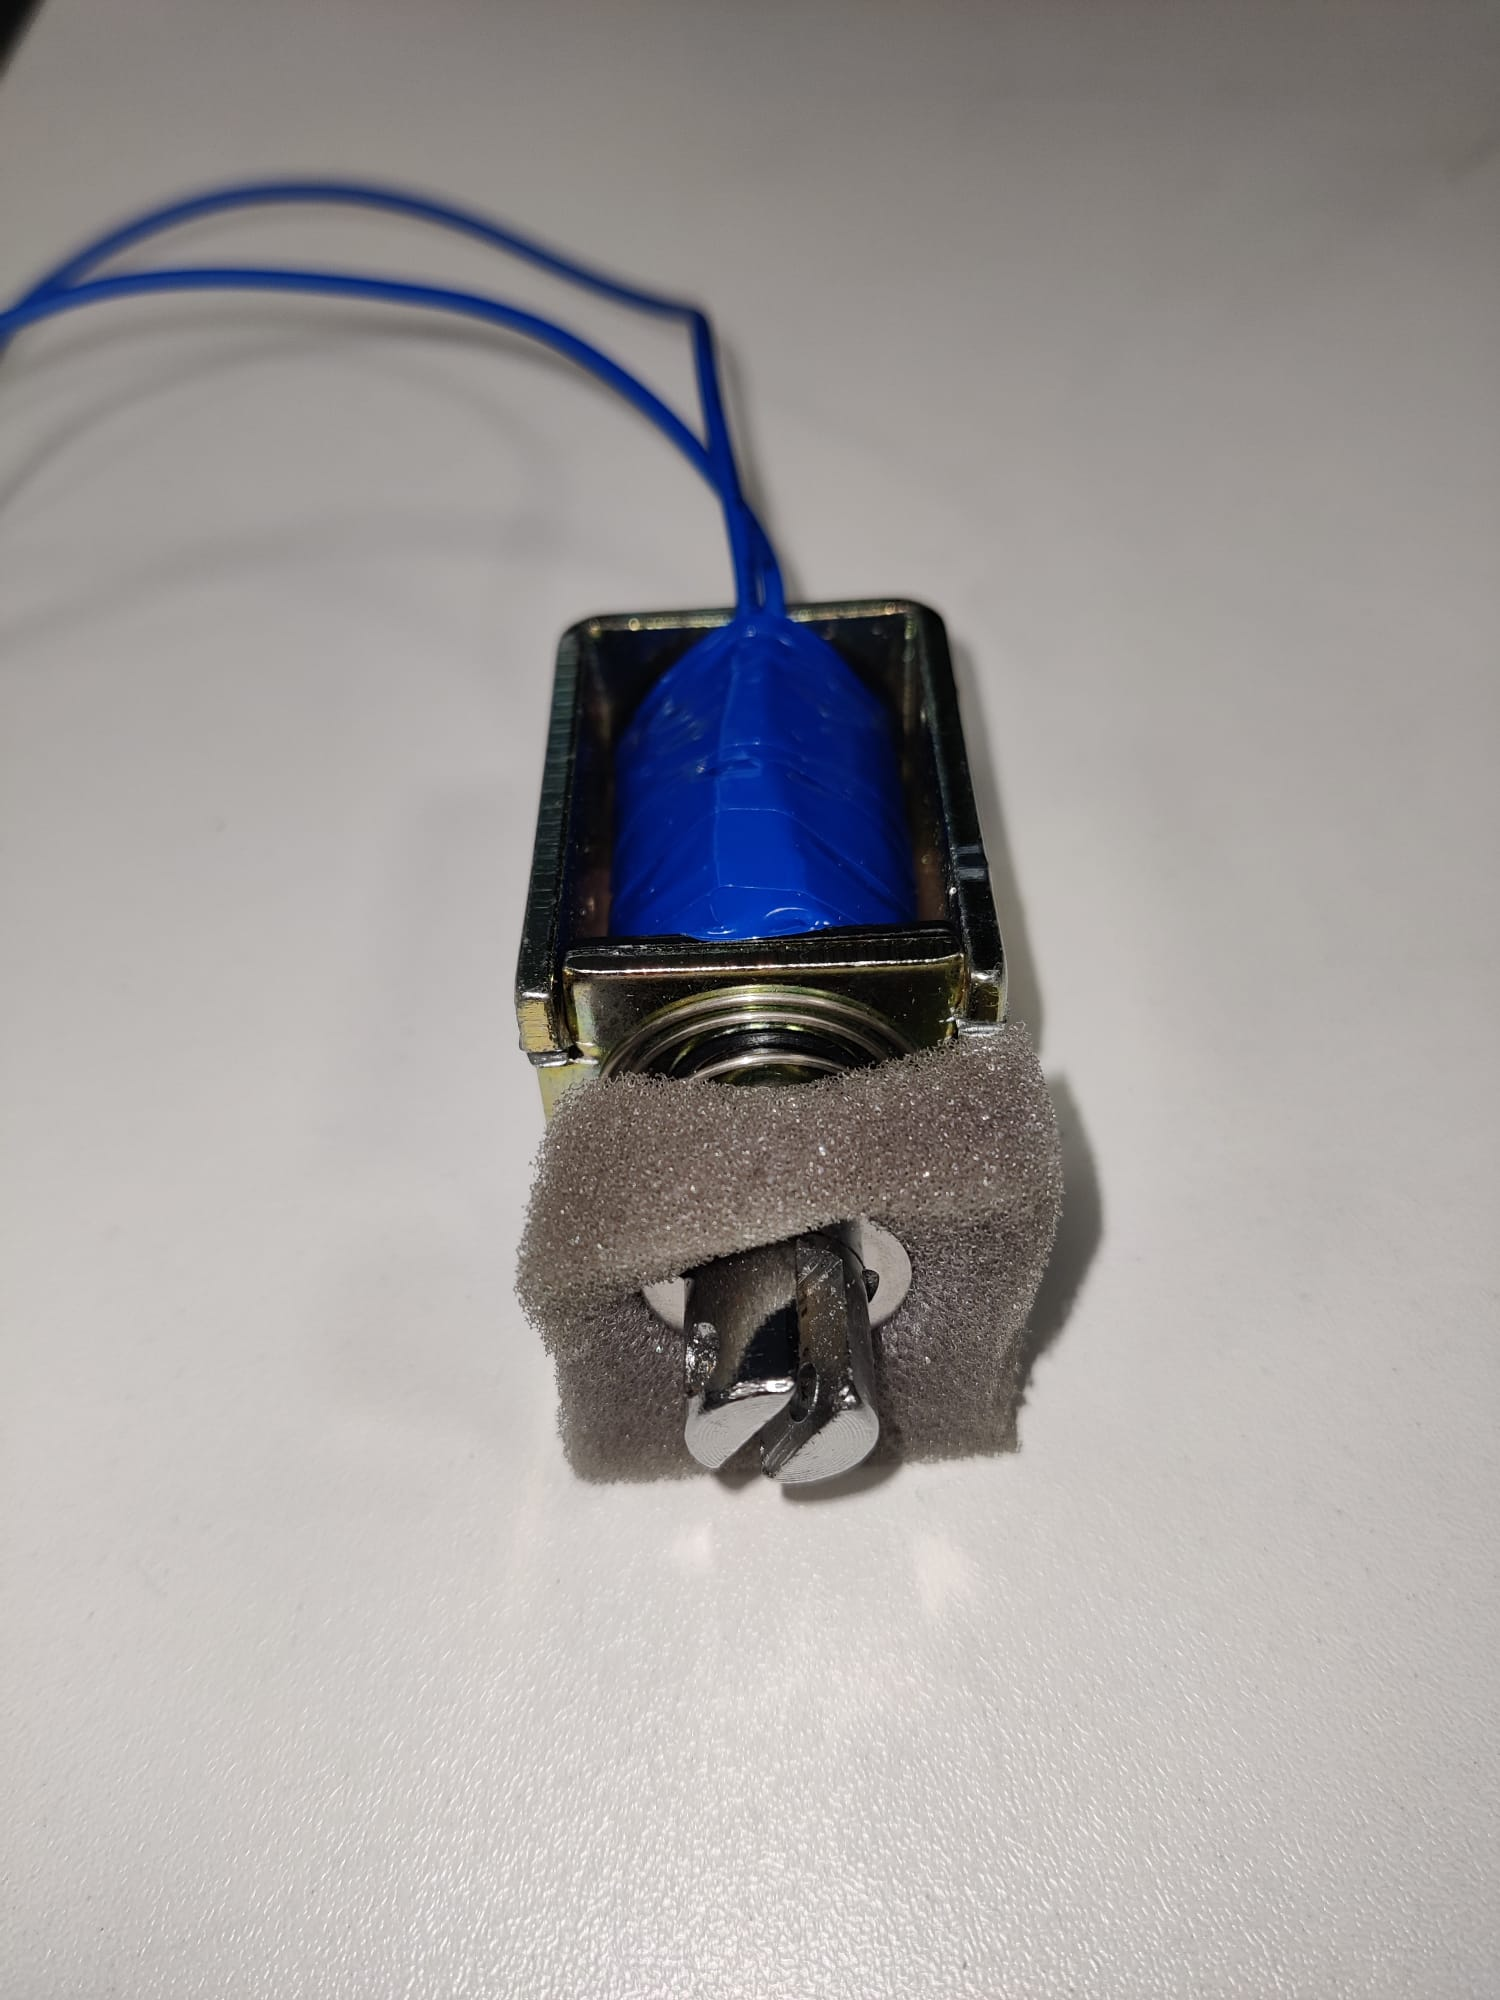
\includegraphics [width=4cm] {img/Daempfung_Schaumstoff}
    \caption{Hubmagnet: Dämpfung mit Schaumstoff}
    \label{fig:schaumstoff}
\end{figure}

\paragraph{Seil (2mm Durchmesser) um den Anker}

Um das \enquote{Problem} der schlechten Ästetik beim Schaumstoff zu beseitigen, wird nun ein 2mm dickes Seil im Inneren des Gehäuses um den Anker gewickelt. \newline
+ Auch hier konnte das Klopfen vollständig beseitigt werden \newline
+ Von außen sieht man keine Veränderung \newline
+ Das Seil scheint ausführlichen Tests nach der Hitzeentwicklung gut Stand zu halten  \newline
- Durch die Dicke des Seils, werden 2mm des Hubs nicht verwendet, weshalb nur noch 8mm übrig bleiben.

\begin{figure}[htbp]
    \centering
    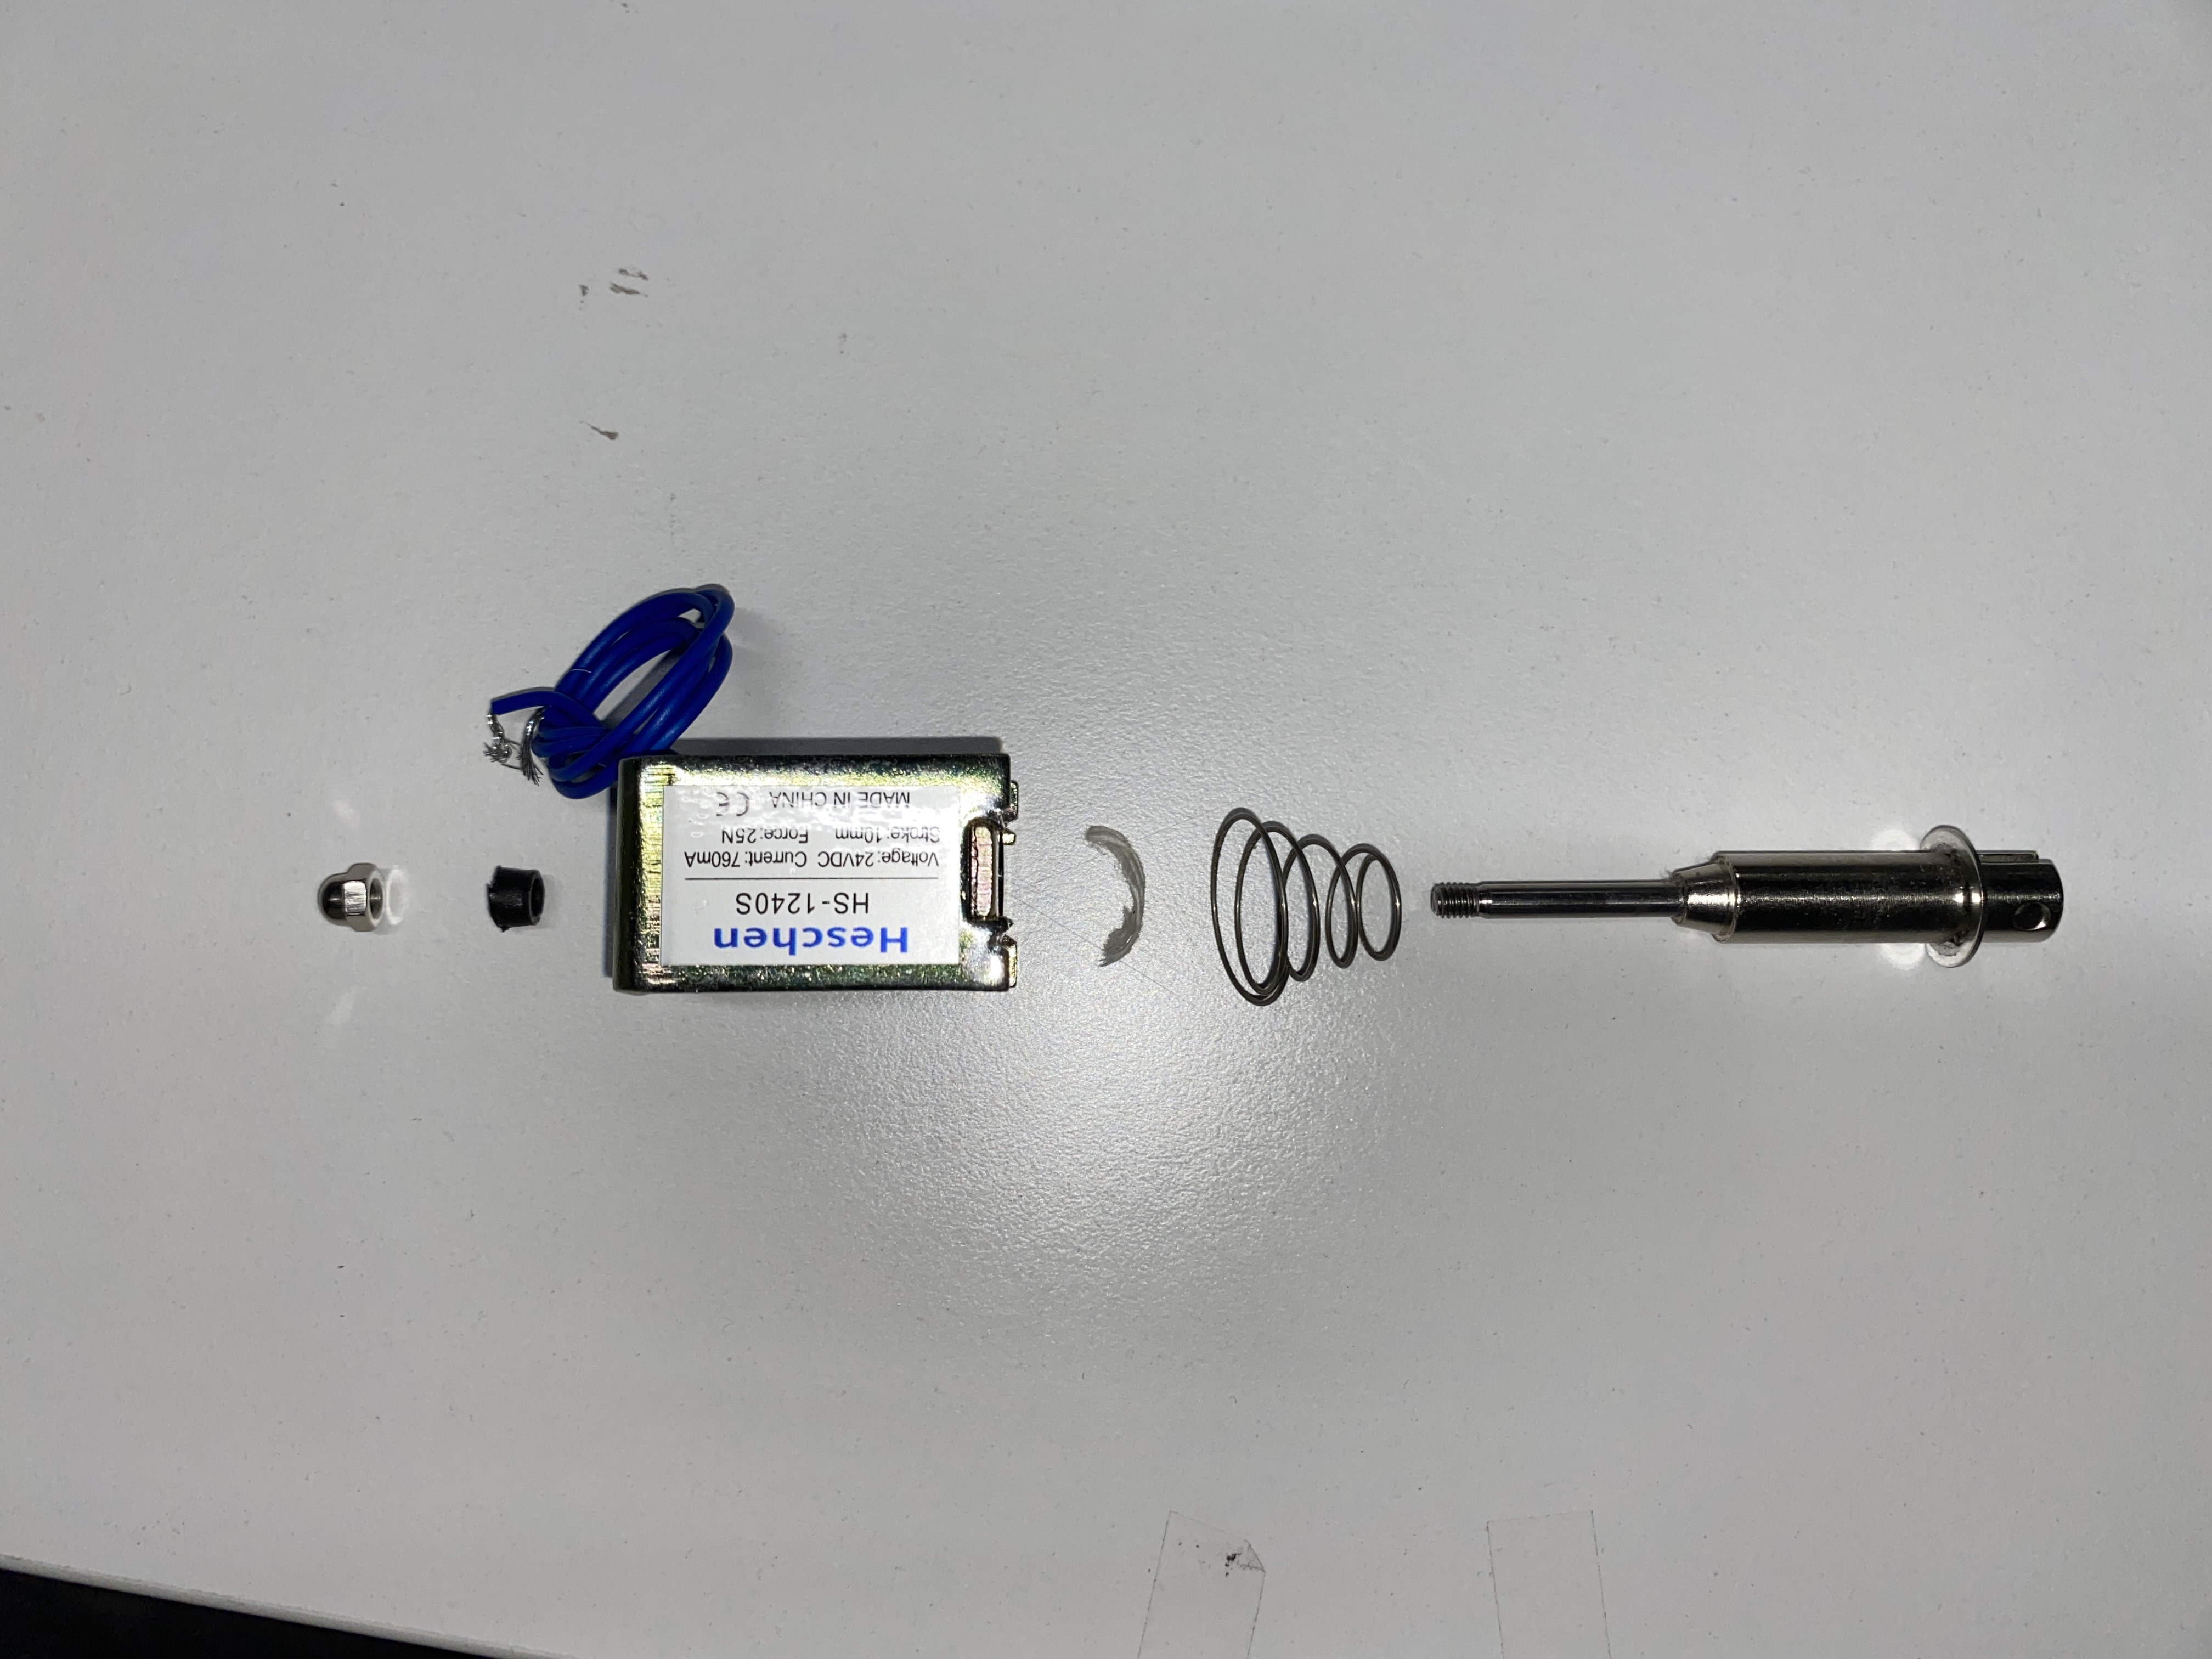
\includegraphics [width=4cm] {img/Hubmagnet_Seil_Daempfung.jpg}
    \caption{Hubmagnet: Dämpfung mit Seil}
\end{figure}


\subsection{Klavieranbau}
Im Rahmen des Protoypen wurde die Elektrik nicht fest am Klavier verschraubt.
Das Brett mit den Hubmagneten wurde stattdessen nur an das Klavier angelehnt, während die Angelschnüre die Verbindung zu den Tasten herstellen.
Gespannt werden die Seile durch eine Schrauben-Mutter Konstruktion (siehe Abschnitt \ref{subsec:VerbindungTastenAktuatoren}).

\subsection{Ergebnisse des Prototypen}
% @TODO(Val):
Der Prototyp des selbstspielenden Klaviers zeigt erfolgreiche Ergebnisse in mehreren Bereichen. Die Implementierung von
8 Tasten funktioniert zuverlässig, wodurch das Klavier in der Lage ist, Töne korrekt wiederzugeben. Seitens der
fertig gelöteten Schaltung könnten 40 Tasten angespielt werden, allerdings haben die Tests sich auf 8 beschränkt.
Ein Großteil der in Kapitel \ref{Zielstellung} definierten Anforderungen konnten von dem Prototypen erfüllt werden.
Zusätzlich erweist sich die Klangdämpfung, dort wo sie eingesetzt wird, als effektiv. \newline
Ein großer Teil, der fehlt, sind Sicherheitskonzepte, weshalb es nicht unbeaufsichtigt betrieben
werden sollte, sowie die Fertigstellung der Schaltung für die zweite Hälfte der Tasten.

Für die mögliche Fertigstellung des Prototypen, muss der Zeitaufwand betrachtet werden.
Von der Umsetzung her ist nur die hälfte des Klaviers anspielbar. Das bedeutet, dass folgendes noch zu tun ist:
\begin{itemize}
    \item Löten der Schaltung für 48 Solenoids
    \item Löten der Anschlussblöcke: 76 Stück
    \item Abisulierung der Hubmagnete für 48 Stück
    \item Fertigstellung des Brettes für die Befästigung der Hubmagnete (Bohren) und die Befästigung
    \item Verbindung zwischen Hubmagneten und Tasten für 76 Stück
    \item Klangdämpfung für 86 Hubmagneten
\end{itemize}

Die Zeiteinschätzung kann gut auf den bisherigen Arbeiten basieren. Das Löten und Abisulieren der Schaltung für
40 Hubmagnete, benötigte etwa 40 Stunden. Die Befästigung der Magnete und die Verbindung mit den Tasten wird auf
mindestens zwei Stunden Arbeit herauslaufen.
Zusätzlich wird mindestens eine Stunde (tendenziell eher 2) für die Klangdämpfung benötigt werden.

Damit beläuft sich die Fertigstellung des Prototypen auf mindestens weitere 44 Stunden. Dazu kommt, dass der Prototyp
noch ausführlich getestet werden muss und gegebenenfalls Fehler die beim Löten o.ä. aufkommen behoben werden müssen.

Der Prototyp wird aus diesem Grund nicht komplett fertiggestellt.
% @TODO(Val): Hier oder bei den Limitationen später genauer beschreiben wie ein Sicherheitskonzept aussehen könnte und warum es gebraucht wird
% @Note(Jay): Steht grad in Limitationen aber wir könnens gerne hier hin ziehen damit hier etwas mehr steht


